%!TEX root = ../thesis.tex

\chapter{Related work}\label{chapter:related_work}

	To better understand the proposed solution in this thesis, this chapter better describes the state of the art and the related work that has been done in this field, both commercially and in research.
	
	% Presentare paper che sono stati rilasciati in questo ambito + progetti europei
	
	% Mostrare prodotti commerciali che sono stati rilasciati per misurare la qualità dell'aria
	
	
	% TODO mantenere le sezioni succesive in questo capitolo o spostare nel successivo?
	
	The solution this thesis focuses on is MegaSense
	
	cina mattina/sera smog
	
	\section{Solutions to detect air pollution}
	
	% Describe these solutions, history, pricing (from the ones that cost a lot and are very reliable to the ones that are cheap and less reliable; a high amount of cheap devices can perform almost as good as a high end device)
	% Describe some solutions that have been previously proposed by other researchears and universities
	
	ArduECO
	
	\begin{figure}
		\centering
		\includegraphics[width=\textwidth]{resources/img/ardueco_circuit}
		\caption{Circuit of the ArduECO prototype, as contained in \cite{ardueco_paper}}
	\end{figure}
	
	\begin{figure}
		\centering
		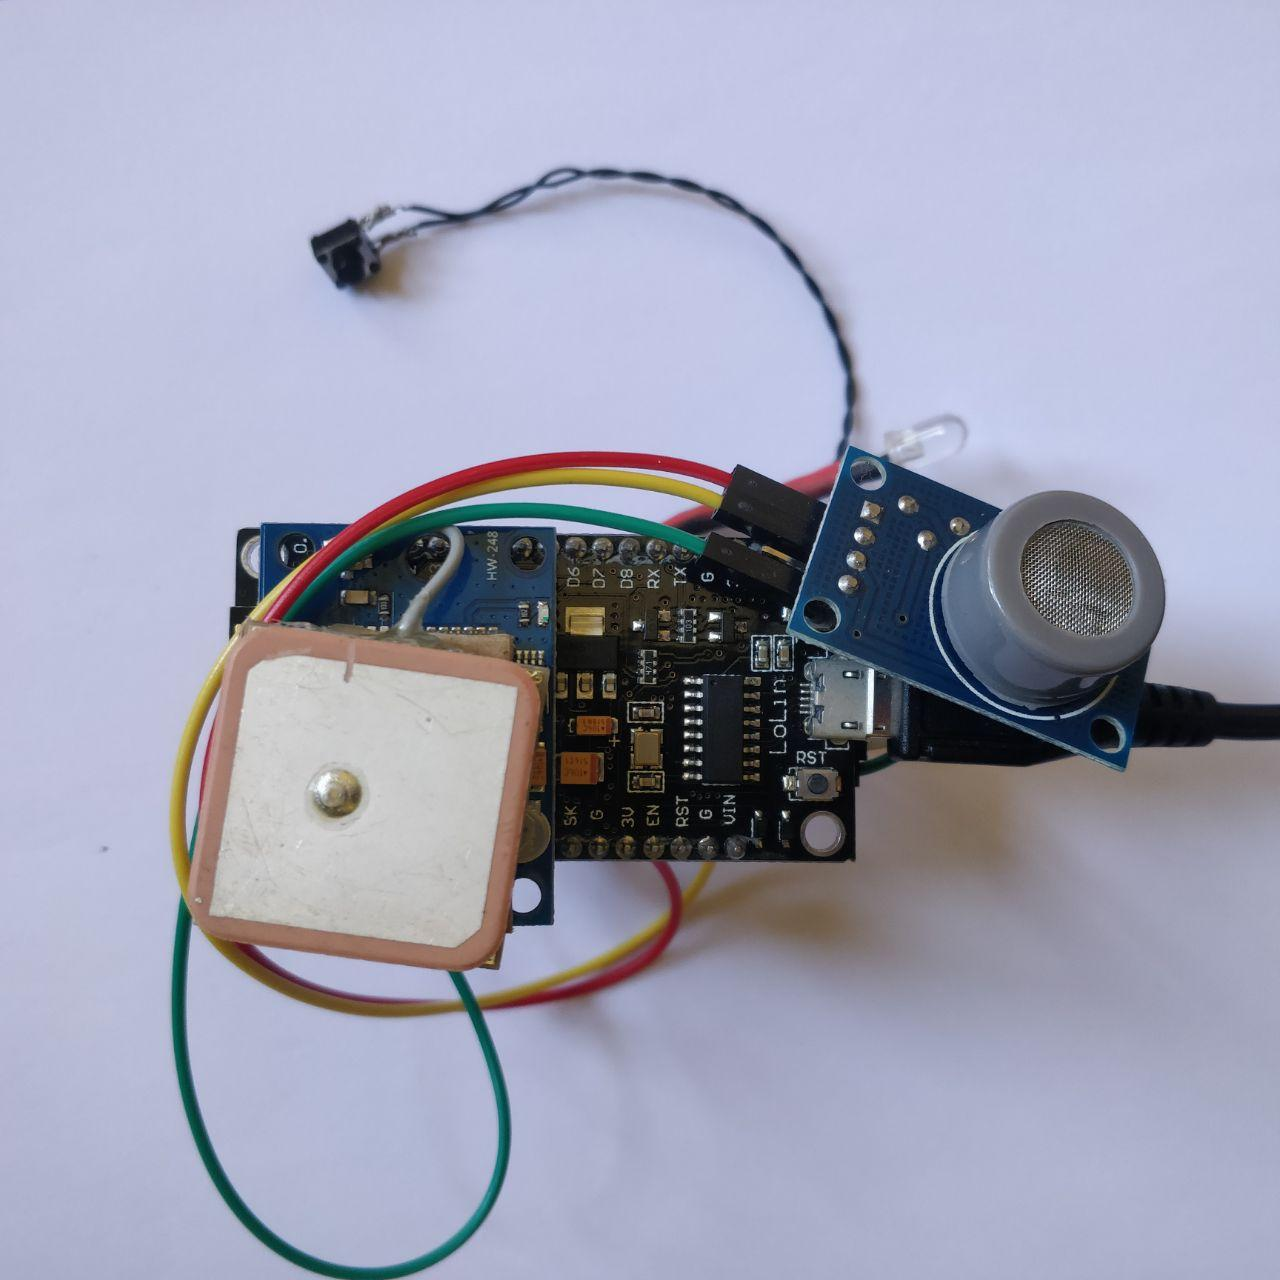
\includegraphics[width=.5\textwidth]{resources/img/ardueco_picture}
		\caption{ArduECO prototype}
	\end{figure}
	
	\section{\megasense}\label{sec:megasense}
	
	% Describe the megasense project, put pictures and explain how it has been developed until now
	
	https://www.megasense.org/
	
	Describe the consortium
	
	HOPE and Megasense
	
	The calibration of the megasense device is made via